%!TEX root = main.tex


%Here you describe a more detailed view of the various parts of the 
%architecture describing how the robot controller or game was designed.

%TODO: Pakkediagram, klassediagram, (sekvens om nødvendig)


\chapter{Design and implementation details}
\label{cha:design_details}

To realise LaHAW, we have decided to use the vanilla Android SDK toolkit. We have chosen not to utilise third party COTS components as we believe that the game is simple enough that any such framework might introduce unwanted constraints.

Central to the game is the \emph{ocean space}, the space where the warships referred to in the title occupy. This ocean space constitutes the main game screen\footnote{Not to be confused with the \emph{main menu} screen from which a game is started.} and is depicted as a grid of tiles.
This grid is programatically drawn directly onto a canvas provided by the Android SDK, which then draws this canvas for the players to see. The game interprets the player's inputs (touching a tile) and calculates behaviour based on the input (determining the tile that was touched and trigger the appropriate reaction).

The other screens that constitutes the game use common interactive elements such as buttons, radio buttons and text boxes to interpret user input. These elements are structured using layouts such as \texttt{LinearLayout} and \texttt{RelativeLayout} in \texttt{XML} files\footnote{WTF is XML?}, also provided by the Android SDK. The user interface in these screens are deliberately simple in terms of design, as the main focus for this project is the underlying architecture.

Audio is implemented using the built in \texttt{MediaPlayer} library in Android, and sound is played when the \texttt{OnTouch} method is triggered in \texttt{GameState}.


Below we will detail the main aspects of our implementation of our two main architectrual patterns.

The first of the two main architecture pattern implemented in LaHAW is \emph{Model-View-Controller}. Because of this, the different classes are seperated into model, view and controller packages. Additionally, the game contains packages for listeners and states.

\begin{figure}[ht]
    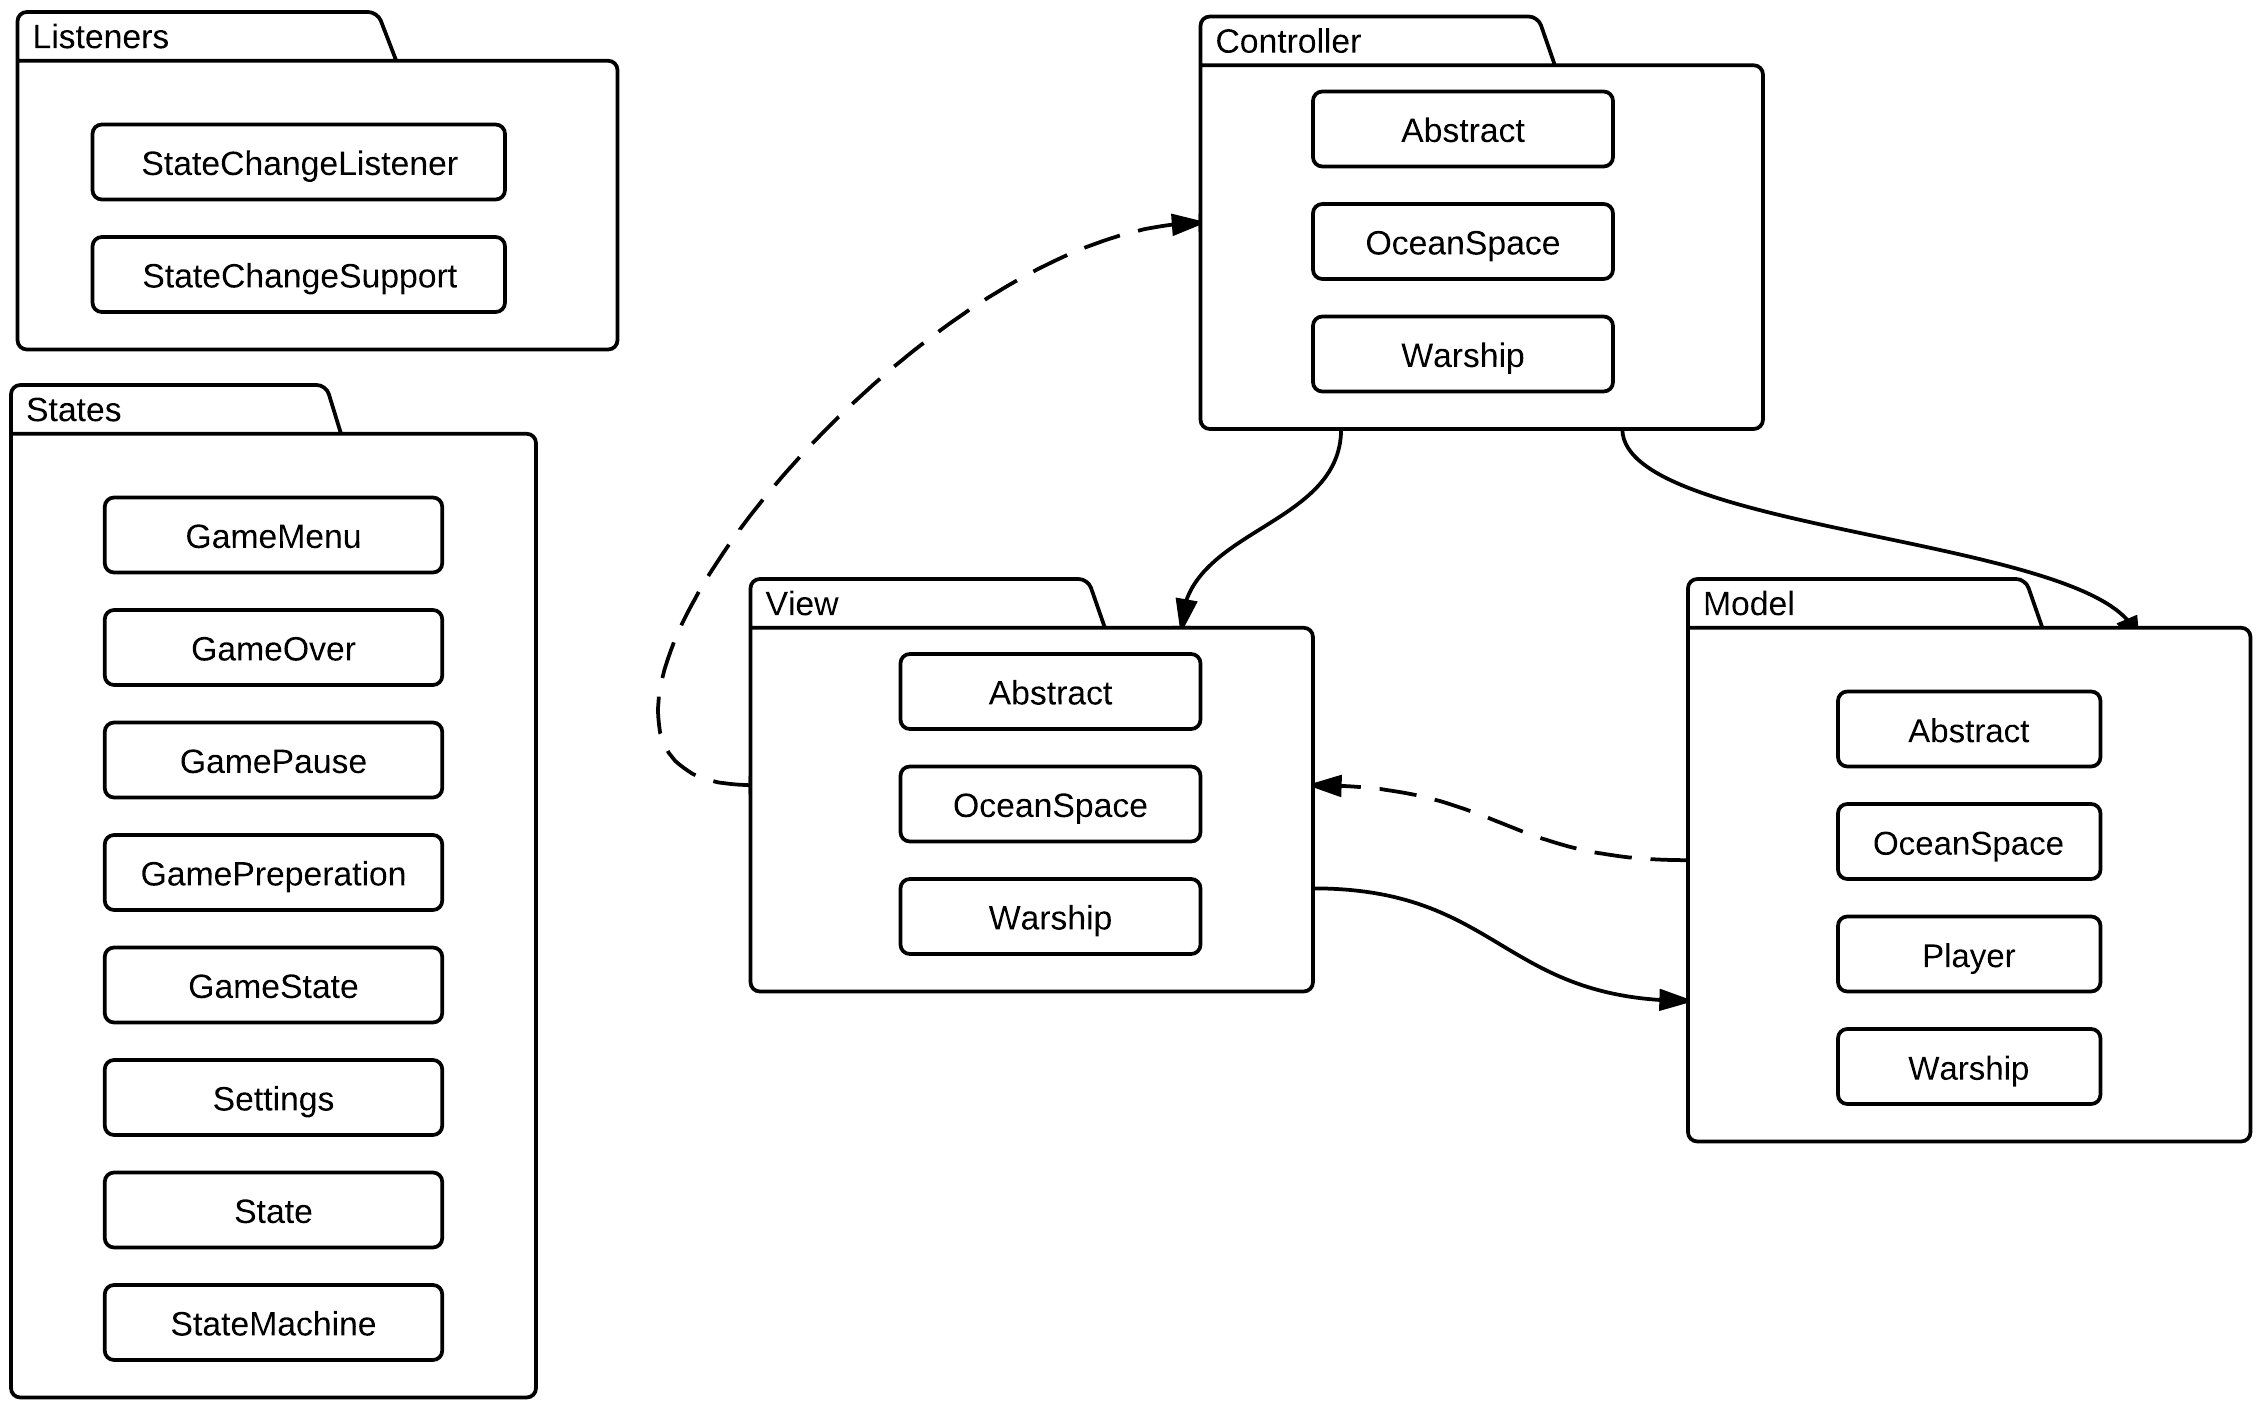
\includegraphics[width=\textwidth]{img/PackageDiagram.png}
    \caption{Package Diagram}
    \label{fig:PackageDiagram}
\end{figure}

Each package contain either the models, views or controllers for warships and the ocean space. The models inherit listener methods from an abstract class called \texttt{AbstractModel}, while the views and controllers inherit draw methods and controller methods respectively. The latter provide functionality to add and remove connected views and models to a given controller. See the appendix for more detailed diagrams for models \ref{fig:ClassModel}, views \ref{fig:ClassView} and controllers \ref{fig:ClassController}.





The state pattern is the second of the two primary architectural pattern implemented. As we did not use any third party libraries or frameworks to support that pattern, we had to implement this by ourselves. % Gjelder ikke dette _alle_ patterns?
The state package contain states for every scenario in the game: \texttt{GameMenu}; \texttt{GameOver}; \texttt{GamePause}; \texttt{GamePreperation}; and \texttt{GameState}. \texttt{GamePreperation} is a state where the user does the pre-game preparation actions (i.e. positioning and rotating ships). Each state implements common methods from a main class called \texttt{State}. These methods provides support for user interaction, in addition to \texttt{StateMachine} features. % Hvorfor forklares kun én state? Eller var du ikke ferdig?

The \texttt{StateMachine} class acts as as a controller for the different states. These states are stored in a \emph{stack}, where one can both push and pop states to and from, from within each state class. By using the state pattern, transitions between the different scenarios become more effective and intuitive. For further information regarding these state classes, see \ref{fig:ClassState}, where detailed diagrams show the interaction between the relevant classes and the methods these classes contain.

